\documentclass[a4paper,11pt]{article}

\usepackage[utf8]{inputenc}

\usepackage{pgfplots}


\begin{document}

\title{
    \textbf{Quick sort an array and a linked list}
    
}
\author{Mahdi Nazari}
\date{October 2022}

\maketitle  
\section*{Introduction}
In this assignment a new sorting algorithm will be presented namely quick sort. Quick sort as it called has a better performance regard to the execution time compared to the other sorting algorithms. Quick sort can be implemented on an array of elements or elements in a linked list. In this work quick sort will be implemented on both of these data structures and to get a clear picture of which implementation is efficient regard to execution time a fairly benchmark will be done and the result will be disused in the conclusion part.  

\section*{Quick sort an array}
For quick sorting an array we need to implement two methods in the quick sort class, namely sort and partition. sort method takes three parameters an array, a low index and high index. This means that we want that an array should be sorted from a low index to a high index. In the sort method we have to keep track of when the low index and high index is the same this means that one element in the array should be sorted and this requires no job since an array with one element is already sorted. In other cases a pivot element should be chosen in the array and in this case we choose the first element in the array as a pivot element.\newline
Then we need another method to get the array be ordered as follows: elements smaller or equal to the pivot element, pivot element and the elements larger than the pivot element. This method will be called partition and will take four parameters, an array, low index, high index and a pivot element. In the partition two new pointers will be declared which will be called leftPointer and rightPointer and these pointers will point to the low index respective high index. Then leftPointer will be incremented as long as leftPointer is smaller than the rightPointer and the elements that the pointer points to is smaller or equal to the pivot element and leftPointer has not passed the end of the sequence which is high index. In the same way the rightPointer will be decremented as long as rightPointer is larger than the leftPointer and the elements that this pointer points to is larger than the pivot element and rightPointer has not reached the edge of the sequence which is low index. These two condition will be implemented with two while-loops inside a third while-loop. The partition method is as below:

 \begin{verbatim}
  public static int partition(int[] array, int lowIndex, int highIndex, int pivot){
            int leftPointer = lowIndex;
            int rightPointer = highIndex;
            while (leftPointer < highIndex && rightPointer > lowIndex){
                while(array[leftPointer] <= pivot && leftPointer < highIndex){	 
                leftPointer++; }
                while(array[rightPointer] > pivot && rightPointer > lowIndex){ 	
                rightPointer--; }
                if(leftPointer > rightPointer){ 	
                break; }
                swap(array, leftPointer, rightPointer);
            }
            swap(array, rightPointer, lowIndex);
            return rightPointer;
        }
   \end{verbatim} 
 When the program is outside of the two inner while-loops two scenarios are possible, either the leftPointer and rightPointer are pointing to an element that is larger respective smaller than the pivot element or leftPointer is not longer less than the rightPointer that means they have passed each others. If the first scenario is relevant the program should swap the elements on leftPointer and rightPointer otherwise the second scenario is relevant and it means that the leftPointer and rightPointer has passed each others and the whole elements that they have passed is less or equal to the pivot element and respective larger than the pivot element. The last operation is to swap the pivot element with the rightPointer that is pointing to an element that is less than the pivot element and return the rightPointer which is pointing to the pivot element.\newline
 
 After partition we get an array which ordered as follows: a sequence of elements less or equal to the pivot element, pivot element and a sequence of elements larger than the pivot element. Now the rightPointer which has been returned from the partition points to pivot element which is in the right place and to sort the whole sequence we need to sort these two subsequences recursively. To do this we call the sort method inside sort method first by parameters array, low index, rightPointer -1 to get the left subsequence sorted and then by array, rightPointer+1, high index to get the right subsequence to be sorted. Sort method is as follows:  
 
    \begin{verbatim}
    public static void sort(int[] array, int lowIndex, int highIndex){
        if(lowIndex >= highIndex){ 		return;}
        int pivot = array[lowIndex];
        int rightPointer = partition(array, lowIndex, highIndex, pivot);
        sort(array, lowIndex, rightPointer-1);
        sort(array, rightPointer+1, highIndex);
    }
    \end{verbatim}  
  
 \section*{Quick sort a linked list}
Quick sort can be implemented on a sequence of elements in a linked list. The principle is the same as quick sorting an array. We still need two methods in the quick sort class as sort and partition. The parameter in the sort and partition will be two pointers as head and end which points to the head and the end of the list. But in the partition we do not need to keep track of the indices. \newline

 Even in a linked list we take the first element or head as pivot. Then we traverse in the list by two pointers, current and previous. Current initially points to the next element after head and previous points to the head. During traversing if the element that current pointer points to is smaller than the pivot element we swap the data of the next element that previous pointer points to with the current elements data. When we have traversed in the list the previous pointer will point to an element that is smaller than the pivot element. We swap the pivot element with the element that previous pointer points to and then we get a sequence of elements which is ordered as follows: a sequence of elements that is less than the pivot element, pivot element and a sequence of elements that is equal or larger than the pivot element.Then the previous pointer which points to the pivot element will be returned to sort method and will be called as newPivot.  \newline

In the sort method the program will sort these two subsequence of lists in the left and right of newPivot by calling sort method recursively and first by parameter head, newPivot to sort the left subsequence list and then by newPivot.next and end to sort the right subsequence of the list. The sort method in linked list is as follows:


  \begin{verbatim}
    public static void QuickSort(Node head, Node end){
        if(head == end || head == null || end == null){
            return;
        }
        Node newPivot = partition(head, end);
        QuickSort(head, newPivot);
        QuickSort(newPivot.next, end);
    }
    \end{verbatim}  
 
 
 \section*{Benchmark}
Now it is time to benchmark these two implementations. Since sorting a sequence of elements depends on how the elements is ordered we need to send the same sequence of elements as an array and linked list to these two implementations. To do this an array of the integer data type was arranged randomly. The same array was converted to a linked list. Now we send an array to QuickSort.Array and a corresponding linked list of that array to QuickSort.LinkedList. The execution time will be calculated every time these two sort methods are called. Benchmark was performed with 10 different arrays size and 10 corresponding linked lists of those arrays. The result is as the table below: 

  \begin{table}[h]
\begin{center}
\begin{tabular}{l|S|l}
\textbf{Number } & \textbf{QS Array}  & \textbf{QS Linked List} \\
\hline
  100      &  732 &77\\
  1000      &  1230 & 526\\
  10000      &  2365& 2462\\
  20000      &  2064  & 2024\\
  30000      &  2544 & 2727\\
  50000      & 3658 &4692\\
  80000      &  6299 & 7358\\
  100000      &  6595& 9625\\
  120000      &  7717 & 10637\\
  200000     &  12652  & 20002\\

\end{tabular}
\caption{The execution time of quick sorting an array of elements and its corresponding linked list with different sizes. Time in us}\newline
\label{tab:table1}
\end{center}
\end{table}\newline

 \subsection*{Conclusion}
The result from benchmarking is mostly in the line with our hypothesis that quick sorting a linked list should take longer time than quick sorting an array. This is because of the differences between memory allocation for each of these data structures and the overhead that it causes. All elements in an array is stored as a block in the memory and access operation for each element can be done in constant time. But elements in a linked list can be stored in different parts of memory and therefore the time for accessing each element is proportional to O(n). Since in quick sort we do use many random access operation this cause a longer execution time for quick sorting a linked list compared to quick sorting an array. \newline

The two first raws in the table shows that the execution time is shorter for quick sorting a linked list than quick sorting an array. This is very strange result which is in opposite to our hypothesis and I am very insure about the reason. But a reason for this result can be that quick sorting a shorter data set is faster in a linked list than in an array?(or?) Apart from tables two first raws the result approve our hypothesis.\newline

The algorithm for quick sorting an array is the same as algorithm for quick sorting a linked list. Therefore the time complexity of these two implementations are the same and in average proportional to O(n*log n). Quick sort consists of two part, sort and partition. In average the number of partitioning will be proportional to O(log n) and in each level we do some comparison and swap operations which is proportional to O(n). Thus in total the time complexity of quick sort is proportional to O(n logn). O(n logn) is a linear time complexity and a corresponding graph for benchmarking result is as in the graph below: 
   
\begin{center}
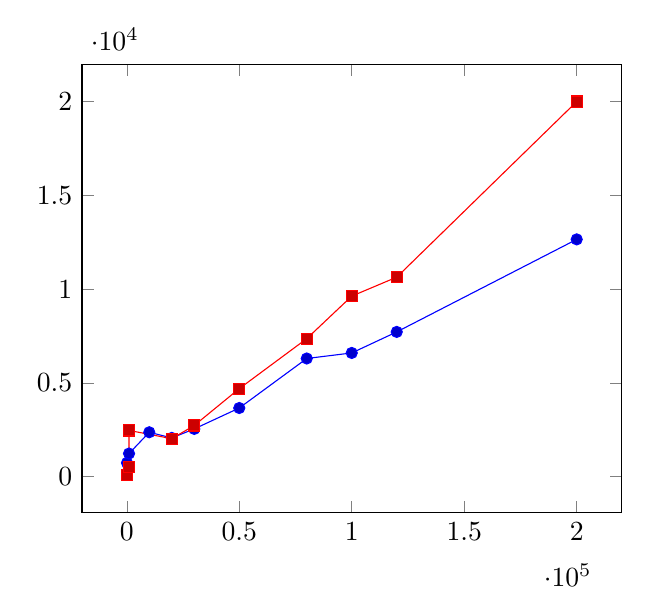
\begin{tikzpicture}
   \begin{axis}
    \addplot coordinates {
    ( 100 ,732)
      ( 1000 , 1230)
      (10000, 2365)
      ( 20000, 2064)
      ( 30000, 2544)
       (50000, 3658)
        (80000, 6299)
       ( 100000, 6595)
       (120000, 7717)
       (200000,12652)
           
    };
     \addplot coordinates {
      ( 100 ,77 )
      ( 1000 , 526)
      (1000, 2462)
      ( 20000, 2024)
      ( 30000, 2727)
       (50000, 4692)
        (80000, 7358)
       ( 100000, 9625)
       (120000, 10637)
       (200000, 20002)
      
           };
      \end{axis}\newline
\end{tikzpicture}\newline
\caption{Graph 1: The result from benchmarking quick sort array(blue graph) vs quick sort linked list(red graph). x-axis is size of data sets, y-axis is execution time in us. }
\end{center}\newline

A the graph shows it clearly the graph for quick sorting an array and quick sorting a linked list are fairly linear which approve the fact that the time complexity for each of these methods is an O(n logn).


\end{document}





















